% Shared preamble of the six stage reports (stages/README.md). Colours and notation are identical in every report.
\documentclass[11pt,a4paper]{article}
\usepackage[margin=2.2cm]{geometry}
\usepackage{amsmath,amssymb,booktabs,graphicx,xcolor,float,caption,subcaption,enumitem,longtable,array}
\usepackage[round]{natbib}
\usepackage[hidelinks]{hyperref}
\usepackage{fancyhdr}
\setlength{\emergencystretch}{2em}
\setlength{\parskip}{3pt}
\definecolor{roigreen}{RGB}{0,160,0}
\definecolor{artred}{RGB}{220,0,0}
\definecolor{maskblue}{RGB}{31,119,180}
\definecolor{ermgrey}{RGB}{110,110,110}
\definecolor{supported}{RGB}{0,120,0}
\definecolor{notsupported}{RGB}{190,0,0}
\newcommand{\ok}{\textcolor{supported}{\textbf{supported}}}
\newcommand{\no}{\textcolor{notsupported}{\textbf{not supported}}}
\newcommand{\mixed}{\textcolor{orange!80!black}{\textbf{partly supported}}}
\newcommand{\roi}{\textcolor{roigreen}{ROI}}
\newcommand{\na}{\textit{n/a}}
\newcommand{\registered}[1]{\textsf{registered before results (#1)}}
\newcommand{\posthoc}[1]{\textsf{post hoc (#1)}}
\pagestyle{fancy}\fancyhf{}\rhead{\small Where the Shortcut Sits --- stage reports}\lfoot{\small\leftmark}\rfoot{\small\thepage}
\newcommand{\stagebox}[1]{\noindent\colorbox{gray!12}{\parbox{\dimexpr\linewidth-2\fboxsep}{\small #1}}\par\medskip}

% generated by make_stage*.py from result files; do not edit
\providecommand{\sFourSmdBeforeHair}{2.127}
\providecommand{\sFourSmdAfterHair}{0.108}
\providecommand{\sFourPairsHair}{398}
\providecommand{\sFourRatioHair}{1.045}
\providecommand{\sFourWorstHair}{lesion area}
\providecommand{\sFourSmdBeforeThy}{0.527}
\providecommand{\sFourSmdAfterThy}{0.045}
\providecommand{\sFourPairsThy}{93}
\providecommand{\sFourRatioThy}{0.998}
\providecommand{\sFourWorstThy}{caliper px log}
\providecommand{\sFourSmdBeforeOv}{0.389}
\providecommand{\sFourSmdAfterOv}{0.079}
\providecommand{\sFourPairsOv}{86}
\providecommand{\sFourRatioOv}{0.958}
\providecommand{\sFourWorstOv}{caliper px log}
\providecommand{\sFourSmdBeforeCap}{2.574}
\providecommand{\sFourSmdAfterCap}{0.231}
\providecommand{\sFourPairsCap}{19}
\providecommand{\sFourRatioCap}{0.611}
\providecommand{\sFourWorstCap}{roi area}
\providecommand{\sFourXHair}{$+0.147$ [$+0.111, +0.185$]}
\providecommand{\sFourMatchHair}{$+0.154$ [$+0.123, +0.186$]}
\providecommand{\sFourMatchFiveHair}{$+0.124$ [$+0.086, +0.162$]}
\providecommand{\sFourMOneHolmHair}{0.000}
\providecommand{\sFourXThy}{$+0.239$ [$+0.196, +0.280$]}
\providecommand{\sFourMatchThy}{$+0.238$ [$+0.186, +0.290$]}
\providecommand{\sFourMatchFiveThy}{$+0.218$ [$+0.165, +0.270$]}
\providecommand{\sFourMOneHolmThy}{0.000}
\providecommand{\sFourXOv}{$+0.170$ [$+0.087, +0.252$]}
\providecommand{\sFourMatchOv}{$+0.163$ [$+0.050, +0.273$]}
\providecommand{\sFourMatchFiveOv}{$+0.152$ [$+0.041, +0.265$]}
\providecommand{\sFourMOneHolmOv}{0.008}
\providecommand{\sFourXCap}{$+0.377$ [$+0.327, +0.426$]}
\providecommand{\sFourMatchCap}{$+0.230$ [$+0.036, +0.434$]}
\providecommand{\sFourMatchFiveCap}{$+0.328$ [$+0.087, +0.573$]}
\providecommand{\sFourUnadjHair}{$+0.154$ [$+0.124, +0.186$]}
\providecommand{\sFourAdjHair}{$+0.156$ [$+0.127, +0.187$]}
\providecommand{\sFourAdjHolmHair}{0.002}
\providecommand{\sFourUnadjThy}{$+0.238$ [$+0.185, +0.291$]}
\providecommand{\sFourAdjThy}{$+0.238$ [$+0.184, +0.291$]}
\providecommand{\sFourAdjHolmThy}{0.002}
\providecommand{\sFourUnadjOv}{$+0.163$ [$+0.058, +0.268$]}
\providecommand{\sFourAdjOv}{$+0.165$ [$+0.056, +0.273$]}
\providecommand{\sFourAdjHolmOv}{0.002}
\providecommand{\sFourNATwoOK}{3}
\providecommand{\sFourNATwo}{3}
\providecommand{\sFourTIHair}{$+0.253$ [$+0.214, +0.293$]}
\providecommand{\sFourTNHair}{$+0.204$ [$+0.164, +0.244$]}
\providecommand{\sFourNThreeHair}{$+0.049$ [$+0.026, +0.072$]}
\providecommand{\sFourTBalHair}{$-0.052$ [$-0.071, -0.033$]}
\providecommand{\sFourShareHair}{81\%}
\providecommand{\sFourTIThy}{$+0.277$ [$+0.256, +0.298$]}
\providecommand{\sFourTNThy}{$+0.145$ [$+0.130, +0.161$]}
\providecommand{\sFourNThreeThy}{$+0.132$ [$+0.116, +0.148$]}
\providecommand{\sFourTBalThy}{$-0.016$ [$-0.025, -0.007$]}
\providecommand{\sFourShareThy}{52\%}
\providecommand{\sFourTIOv}{$+0.074$ [$+0.044, +0.104$]}
\providecommand{\sFourTNOv}{$+0.052$ [$+0.021, +0.084$]}
\providecommand{\sFourNThreeOv}{$+0.022$ [$-0.002, +0.048$]}
\providecommand{\sFourTBalOv}{$-0.011$ [$-0.025, +0.002$]}
\providecommand{\sFourShareOv}{71\%}
\providecommand{\sFourTICap}{$+0.497$ [$+0.427, +0.567$]}
\providecommand{\sFourTNCap}{$+0.459$ [$+0.383, +0.535$]}
\providecommand{\sFourNThreeCap}{$+0.037$ [$-0.017, +0.093$]}
\providecommand{\sFourTBalCap}{$-0.032$ [$-0.068, +0.004$]}
\providecommand{\sFourShareCap}{92\%}
\providecommand{\sFourShareMin}{52\%}
\providecommand{\sFourShareMax}{92\%}
\providecommand{\sFourNNThreePos}{2}
\providecommand{\sFourDpErmInHair}{0.340}
\providecommand{\sFourDpMaskInHair}{0.297}
\providecommand{\sFourMaskCleanInHair}{0.672}
\providecommand{\sFourErmCleanInHair}{0.776}
\providecommand{\sFourMaskRevOutHair}{0.716}
\providecommand{\sFourMaskCorrOutHair}{0.716}
\providecommand{\sFourMaskCleanOutHair}{0.716}
\providecommand{\sFourNRecipHair}{860}
\providecommand{\sFourDpErmInThy}{0.206}
\providecommand{\sFourDpMaskInThy}{0.271}
\providecommand{\sFourMaskCleanInThy}{0.801}
\providecommand{\sFourErmCleanInThy}{0.708}
\providecommand{\sFourMaskRevOutThy}{0.846}
\providecommand{\sFourMaskCorrOutThy}{0.846}
\providecommand{\sFourMaskCleanOutThy}{0.846}
\providecommand{\sFourNRecipThy}{1800}
\providecommand{\sFourDpErmInOv}{0.037}
\providecommand{\sFourDpMaskInOv}{0.116}
\providecommand{\sFourMaskCleanInOv}{0.755}
\providecommand{\sFourErmCleanInOv}{0.723}
\providecommand{\sFourMaskRevOutOv}{0.750}
\providecommand{\sFourMaskCorrOutOv}{0.750}
\providecommand{\sFourMaskCleanOutOv}{0.750}
\providecommand{\sFourNRecipOv}{348}
\providecommand{\sFourDpErmInCap}{0.238}
\providecommand{\sFourDpMaskInCap}{0.551}
\providecommand{\sFourMaskCleanInCap}{0.871}
\providecommand{\sFourErmCleanInCap}{0.787}
\providecommand{\sFourMaskRevOutCap}{0.914}
\providecommand{\sFourMaskCorrOutCap}{0.914}
\providecommand{\sFourMaskCleanOutCap}{0.914}
\providecommand{\sFourNRecipCap}{340}
\providecommand{\sFourSensdinoFiveOneEightmainThyroid}{$+0.239$ [$+0.196, +0.280$]}
\providecommand{\sFourSensdinoFiveOneEightsenspxFiveZeroThyroid}{$+0.244$ [$+0.199, +0.289$]}
\providecommand{\sFourSensdinoFiveOneEightsensstrictlocThyroid}{$+0.212$ [$+0.164, +0.259$]}
\providecommand{\sFourSensdinoFiveOneEightmainOvary}{$+0.170$ [$+0.087, +0.252$]}
\providecommand{\sFourSensdinoFiveOneEightsenspxFiveZeroOvary}{$+0.188$ [$+0.108, +0.266$]}
\providecommand{\sFourSensdinoFiveOneEightsensstrictlocOvary}{$+0.196$ [$+0.117, +0.277$]}
\providecommand{\sFourSensdinoFiveOneEightmainCapsule}{$+0.377$ [$+0.327, +0.426$]}
\providecommand{\sFourSensdinoFiveOneEightsensstrictBCapsule}{$+0.255$ [$+0.153, +0.349$]}
\providecommand{\sFourEmbThyroid}{$+0.235$ [$+0.193, +0.275$]}
\providecommand{\sFourEmbOvary}{$+0.157$ [$+0.053, +0.255$]}
\providecommand{\sFourEmbCapsule}{$+0.353$ [$+0.296, +0.410$]}
\providecommand{\sFourEstN}{204}
\providecommand{\sFourEstLost}{3}
\providecommand{\sFourEstGained}{0}
\providecommand{\sFourEstMed}{1.63}
\providecommand{\sFourRegPre}{\texttt{5ef3228}, 2026-09-26 14:57}
\providecommand{\sFourRegRevTwo}{\texttt{29cd0da}, 2026-09-27 18:56}
\providecommand{\sFourRegRevThree}{\texttt{85da735}, 2026-09-27 23:43}
\providecommand{\sFourRegFinal}{\texttt{c45d482}, 2026-09-28 00:35}

\title{\textbf{Stage 4 --- Causal checks and the bootstrap correction}\\[3pt]\large Where the Shortcut Sits: supervisor meeting 4 of 6}
\author{}
\date{Report generated from the repository on \today}
\begin{document}
\maketitle
\stagebox{\textbf{In one sentence.} The real-artifact crossover survives covariate matching and regression adjustment
in all three cohorts where matching is feasible (A2: \sFourNATwoOK{} of \sFourNATwo{} supported); moving the same real
artifact inside and outside the ROI of the same image produces a crossover too, but a neutral paste of the same shape
reproduces most of it, so only a small part --- significant for hair and thyroid calipers --- is attributable to the
artifact's content. The bootstrap correction widened intervals by a median factor of \sFourCMedian{} and changed
\sFourCChanged{} of \sFourCRows{} significance verdicts.}
% Shared notation. Each stage defines \notY, \notA, \notROI, \notCross, \notCI and \notExtra before \input-ing this
% file, so that a report only names the cohorts and quantities it has already introduced.
\section*{Notation}
\begin{tabular}{p{3.2cm}p{11.8cm}}
$Y\in\{0,1\}$ & diagnosis: \notY. \\
$A\in\{0,1\}$ & artifact present: \notA. \\
ROI & region of interest: \notROI; drawn in \textcolor{roigreen}{green}; artifacts in \textcolor{artred}{red}. \\
$r$ & overlap $|\text{artifact}\cap\text{ROI}|/|\text{artifact}|$. Trap~A: $r\ge0.5$ (artifact in the ROI); Trap~B: $r<0.1$ (outside). \\
Environments & training and correlated test $P(A{=}1\mid Y{=}1)=0.9$, $P(A{=}1\mid Y{=}0)=0.1$; reversed test 0.1/0.9; clean test: artifact independent of $Y$ (real artifacts: half of each class) or absent (synthetic artifacts). \\
ERM, mask & linear head on the frozen features of the original image / of the ROI-masked image. \\
Crossover & \notCross \\
CI & \notCI \\
$|\Delta p|$ & same-head counterfactual sensitivity: change of the predicted probability when the artifact is inserted into the same image. \\
\notExtra
\end{tabular}


\section{Where we are}
Stage~3 showed a positive crossover with real artifacts. Real artifacts are not placed at random: in dermoscopy, hair
lies on large lesions more often than on small ones; in thyroid ultrasound, calipers inside the nodule are drawn on
larger, more heavily measured nodules. Artifact-based debiasing studies in dermoscopy make the same point about where artifacts occur
\citep{bissoto2020debiasing,nauta2022uncovering}. The crossover could therefore reflect \emph{which images} carry in-ROI artifacts
rather than \emph{where} the artifact lies. This meeting reports the three checks designed to separate the two ---
matching, regression adjustment on the matched sample (A2, new in this round) and transplantation of the same artifact
with a paste-edge control --- and, because it concerns what every interval means, the full consequences of the
bootstrap correction.

\section{Question}
\begin{enumerate}[label=\textbf{Q4\alph*},leftmargin=*]\itemsep1pt
\item Is the crossover explained by measured differences between in-ROI and out-of-ROI artifact images?
\item Does it survive when the artifact is moved within the \emph{same} image, and how much of that is due to the
artifact rather than to pasting something into the image?
\item Which earlier claims change when the uncertainty is estimated correctly?
\end{enumerate}
\paragraph{Why three checks} Matching removes measured imbalance but depends on the chosen covariates; regression on the
matched sample (a doubly robust combination) protects against residual imbalance and model misspecification of either
step alone; transplantation removes image-level confounding altogether but introduces its own artifact --- the paste.
The neutral paste (same mask shape, same compositing, filled with the donor's own clean tissue) measures that paste
effect. Rejected alternatives: inverse-probability weighting (extreme weights with standardised differences above 2 in
dermoscopy and capsule) and synthetic control images (they would test Stage~2 again, not real artifacts).

\section{Methods}
\paragraph{Balance and matching (R1)} Pre-specified covariates per cohort (dermoscopy: lesion area, hair amount, age,
sex, site, source, image size; thyroid: nodule area, caliper pixels, image size, grey level, nodule position; ovary and
capsule analogous). Standardised mean differences (SMD) between Trap~A and Trap~B artifact images; greedy 1:1
nearest-neighbour matching on the logit of a propensity model within label, without replacement, calliper 0.2 SD
(0.05 SD as a stricter sensitivity analysis, R7). A cohort with fewer than 30 matched images per label is infeasible.
\paragraph{Regression adjustment (A2)} For each reversed-test image of the matched sample, the \emph{placement value} of
the masked minus the ERM score (for a positive: the weighted share of negatives ranked below it; for a negative: the
complement of the share of positives ranked above it), so that the class means reproduce the AUROC and the unadjusted
difference between traps equals the crossover exactly (verified per seed). Within each seed, weighted least squares of
this outcome on an intercept, the Trap-B indicator, the label and all matching covariates; the adjusted crossover is
the Trap-B coefficient averaged over seeds. Crossed bootstrap with placement values and regression recomputed in every
replicate (2,000 replicates); Holm over the three cohorts.
\paragraph{Transplant (R2) and neutral paste (R5)} For each artifact-free recipient image, a real artifact instance is
cut from a donor of the same cohort (the donor's mask pixels, largest connected component) and alpha-composited at a
position fully inside and at a position fully outside the recipient's ROI, with a random dihedral transform. The trap
environments are then built as in Stage~1 with the pasted instance as the artifact. The neutral paste keeps the mask
shape, the transform and the compositing but fills the mask with tissue from the donor image at a window that does
not touch its artifact.
\paragraph{Bootstrap correction (A1)} Every archived interval with a regenerated counterpart was compared row by row:
old and new interval, whether ``excludes zero'' changed, width ratio and point-estimate difference.

\section{Experiments}
\begin{table}[H]\centering\scriptsize
\caption{Experiments of this stage. Commit times come from this machine and are not independent proof of order; the final registration was additionally pushed to GitHub before the runs.}\label{tab:exp}
\begin{tabular}{p{3.1cm}p{2.1cm}p{2.4cm}p{3.2cm}p{3.3cm}}\toprule
Experiment & Status & Registration & First commit (local time) & Support criterion \\\midrule
Covariate balance (SMD) and matched traps, M1 & \ok{} registered & REVIEW2 (R1) & \texttt{29cd0da}, 2026-09-27 18:56 & matched crossover CI $>0$, Holm over 3 feasible cohorts \\
Stricter calliper 0.05 SD (R7) & \ok{} registered & REVIEW3 & \texttt{85da735}, 2026-09-27 23:43 & sensitivity, descriptive \\
Real-artifact transplant, T1 & \ok{} registered & REVIEW2 (R2) & \texttt{29cd0da}, 2026-09-27 18:56 & interaction CI $>0$, Holm over 4 \\
Neutral paste (paste-edge control), N3 & \ok{} registered & REVIEW3 (R5) & \texttt{85da735}, 2026-09-27 23:43 & artifact $-$ neutral interaction CI $>0$ \\
Regression-adjusted crossover, A2 & \ok{} registered & FINAL (A2) & \texttt{c45d482}, 2026-09-28 00:35 & adjusted crossover CI $>0$, Holm over 3 \\
Crossed bootstrap everywhere, A1 & \ok{} registered & FINAL (A1) & \texttt{c45d482}, 2026-09-28 00:35 & rewrite claims whose CI now includes 0 \\
Capsule matched analysis & \no{} descriptive & REVIEW2 (R1) & \texttt{29cd0da}, 2026-09-27 18:56 & infeasible under the registered rule \\
\bottomrule\end{tabular}
\end{table}


\section{Results}
\subsection{Imbalance and matching}
The in-ROI and out-of-ROI artifact images differ strongly (Table~\ref{tab:bal}): in dermoscopy the largest SMD is
\sFourSmdBeforeHair{} (\sFourWorstHair: hair lies inside large lesions), in capsule \sFourSmdBeforeCap{}
(\sFourWorstCap). Matching brings the maximum SMD to \sFourSmdAfterHair{} (dermoscopy), \sFourSmdAfterThy{} (thyroid)
and \sFourSmdAfterOv{} (ovary); capsule matching is infeasible (\sFourPairsCap{} pairs in the smaller label, SMD after
matching \sFourSmdAfterCap). The crossover is essentially unchanged by matching (Table~\ref{tab:match}): dermoscopy
\sFourMatchHair, thyroid \sFourMatchThy, ovary \sFourMatchOv; with the stricter calliper \sFourMatchFiveHair,
\sFourMatchFiveThy{} and \sFourMatchFiveOv. Capsule, matched descriptively, gives \sFourMatchCap{} --- lower than the
unmatched \sFourXCap{} and imprecise.
\begin{table}[H]\centering\scriptsize
\caption{Balance of pre-specified covariates between the in-ROI (Trap~A) and out-of-ROI (Trap~B) artifact images, before and after 1:1 nearest-neighbour matching within label (calliper 0.2 SD, pooled standardised mean differences). Registered rule: fewer than 30 matched images per label in either trap makes a cohort infeasible; target max $|$SMD$|\le0.1$ after matching.}\label{tab:bal}
\resizebox{\linewidth}{!}{\begin{tabular}{lccccc}\toprule
Cohort & Least balanced covariate & max $|$SMD$|$ before & after matching & min matched pairs per label & feasible (rule) \\\midrule
ISIC hair & lesion\_area & 2.127 & 0.108 & 398 & yes \\
Thyroid & caliper\_px\_log & 0.527 & 0.045 & 93 & yes \\
Ovary & caliper\_px\_log & 0.389 & 0.079 & 86 & yes \\
Capsule & roi\_area & 2.574 & 0.231 & 19 & \textbf{no} \\
\bottomrule\end{tabular}}
\end{table}

\begin{table}[H]\centering\scriptsize
\caption{Crossover before and after covariate matching (reversed-test AUROC, crossed 95\% CIs). The 0.05 SD calliper is the stricter sensitivity analysis of the third review (R7).}\label{tab:match}
\resizebox{\linewidth}{!}{\begin{tabular}{lcccc}\toprule
Cohort & Crossover, all images & matched (0.2 SD) & matched (0.05 SD) & M1 (Holm, 3) \\\midrule
ISIC hair & $+0.147$ [$+0.111, +0.185$] & $+0.154$ [$+0.123, +0.186$] & $+0.124$ [$+0.086, +0.162$] & \ok \\
Thyroid & $+0.239$ [$+0.196, +0.280$] & $+0.238$ [$+0.186, +0.290$] & $+0.218$ [$+0.165, +0.270$] & \ok \\
Ovary & $+0.170$ [$+0.087, +0.252$] & $+0.163$ [$+0.050, +0.273$] & $+0.152$ [$+0.041, +0.265$] & \ok \\
Capsule & $+0.377$ [$+0.327, +0.426$] & $+0.230$ [$+0.036, +0.434$] & $+0.328$ [$+0.087, +0.573$] & descriptive (infeasible) \\
\bottomrule\end{tabular}}
\end{table}

\begin{table}[H]\centering\scriptsize
\caption{Per-covariate balance, thyroid and ovary (pooled over labels). The dermoscopy and capsule tables (17 and 20 covariates) are in \texttt{results/rerun\_2026-09-28/review2/R1\_balance.csv}.}\label{tab:baldet}
\begin{tabular}{lccc}\toprule
Cohort & Covariate & SMD before & SMD after \\\midrule
Thyroid & roi\_area & $+0.395$ & \na \\
Thyroid & caliper\_px\_log & $+0.527$ & \na \\
Thyroid & width & $-0.143$ & \na \\
Thyroid & height & $-0.123$ & \na \\
Thyroid & mean\_grey & $+0.183$ & \na \\
Thyroid & roi\_centroid\_row & $+0.060$ & \na \\
Ovary & roi\_area & $+0.320$ & \na \\
Ovary & caliper\_px\_log & $+0.389$ & \na \\
Ovary & width & $-0.298$ & \na \\
Ovary & height & $+0.047$ & \na \\
Ovary & mean\_grey & $+0.107$ & \na \\
Ovary & subtype=0.0 & $+0.149$ & $-0.079$ \\
Ovary & subtype=1.0 & $+0.059$ & $+0.072$ \\
Ovary & subtype=2.0 & $-0.159$ & $-0.012$ \\
Ovary & subtype=3.0 & $-0.054$ & $+0.000$ \\
Ovary & subtype=4.0 & $-0.022$ & $+0.024$ \\
Ovary & subtype=6.0 & $+0.024$ & $+0.056$ \\
Ovary & subtype=7.0 & $-0.020$ & $-0.062$ \\
\bottomrule\end{tabular}
\end{table}


\subsection{Regression adjustment on the matched sample (A2)}
The adjusted crossover equals the unadjusted one to the third decimal in every cohort (Table~\ref{tab:a2}): dermoscopy
\sFourAdjHair{} (unadjusted \sFourUnadjHair), thyroid \sFourAdjThy{} (\sFourUnadjThy), ovary \sFourAdjOv{}
(\sFourUnadjOv); Holm-adjusted $p$ = \sFourAdjHolmHair, \sFourAdjHolmThy{} and \sFourAdjHolmOv. All \sFourNATwo{} pre-registered tests are supported.
Residual imbalance after matching (up to the per-label maxima in Table~\ref{tab:a2}) does not carry the effect. Capsule
stays descriptive, as registered. What this cannot exclude is an \emph{unmeasured} difference between the images.
\begin{table}[H]\centering\scriptsize
\caption{Regression-adjusted crossover on the matched traps (A2): per-image placement values of the masked minus the ERM score regressed on the Trap-B indicator, the label and all matching covariates, within seed; crossed bootstrap (2,000 replicates). Capsule is not analysed (matching infeasible; descriptive only).}\label{tab:a2}
\resizebox{\linewidth}{!}{\begin{tabular}{lccccccc}\toprule
Cohort & Test images per seed & Covariate columns & Post-matching max $|$SMD$|$ pooled / per label & Unadjusted crossover & Adjusted (doubly robust) & $p$ (Holm, 3) & A2 \\\midrule
ISIC hair & 2960 & 17 & 0.108 / 0.164 & $+0.154$ [$+0.124, +0.186$] & $+0.156$ [$+0.127, +0.187$] & 0.002 & \ok \\
Thyroid & 2150 & 6 & 0.045 / 0.150 & $+0.238$ [$+0.185, +0.291$] & $+0.238$ [$+0.184, +0.291$] & 0.002 & \ok \\
Ovary & 576 & 11 & 0.079 / 0.140 & $+0.163$ [$+0.058, +0.268$] & $+0.165$ [$+0.056, +0.273$] & 0.002 & \ok \\
\bottomrule\end{tabular}}
\end{table}


\subsection{The same artifact inside and outside the ROI}
\begin{figure}[H]\centering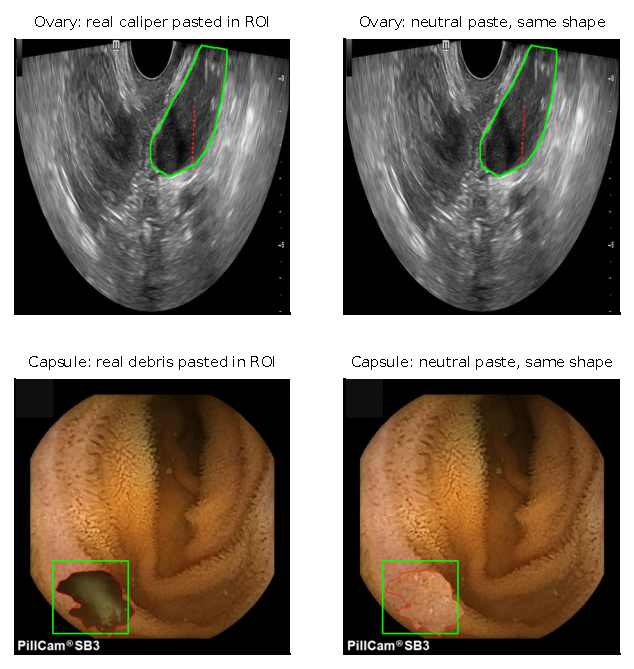
\includegraphics[width=0.62\linewidth]{figures/transplant_examples.pdf}
\caption{Transplant and neutral paste on the same recipient images (openly licensed cohorts; MMOTU, SEE-AI CC BY 4.0).
Left: a real artifact instance pasted inside the ROI (\textcolor{roigreen}{green}; the pasted region outlined in
\textcolor{artred}{red}). Right: the neutral paste --- same mask shape and compositing, filled with artifact-free tissue
from the donor.}\label{fig:tx}\end{figure}
Pasting the same real instance outside versus inside the ROI yields a positive location interaction in every cohort
(Table~\ref{tab:tx}; dermoscopy \sFourTIHair, thyroid \sFourTIThy, ovary \sFourTIOv, capsule \sFourTICap). The neutral
paste, however, reproduces \sFourShareMin{} to \sFourShareMax{} of that interaction (Table~\ref{tab:neutral}): pasting
\emph{anything} into the ROI changes what masking does, because the paste itself is a new, label-correlated pattern
inside the ROI (the environments make the pasted region label-correlated whatever it contains). Only the difference
between the two --- N3, the interaction with the real artifact minus the interaction with the neutral paste --- is
attributable to the artifact's content: dermoscopy \sFourNThreeHair, thyroid \sFourNThreeThy, ovary \sFourNThreeOv{}
and capsule \sFourNThreeCap{} (\sFourNNThreePos{} of 4 excluding zero).
\textbf{Consequently no harm figure from the transplant (for example, the effect of masking with the pasted hair
inside the lesion) is attributed to the real artifact.} The transplant supports the \emph{location} mechanism --- a
label-correlated pattern inside the ROI survives masking --- and N3 shows that the real hair and caliper content adds
to it.
\begin{table}[H]\centering\scriptsize
\caption{Real-artifact transplant (T1): the same real artifact instance, cut from a donor image, pasted outside and inside the ROI of the same artifact-free recipient images. These effects combine the artifact with the paste itself (seam, occluded tissue); Table~\ref{tab:neutral} separates them.}\label{tab:tx}
\resizebox{\linewidth}{!}{\begin{tabular}{lcccc}\toprule
Cohort & mask $-$ ERM, pasted outside ROI & pasted inside ROI & Location interaction & Balanced: interaction \\\midrule
ISIC hair & $+0.178$ [$+0.128, +0.227$] & $-0.075$ [$-0.114, -0.036$] & $+0.253$ [$+0.214, +0.293$] & $-0.052$ [$-0.071, -0.033$] \\
Thyroid & $+0.349$ [$+0.321, +0.379$] & $+0.072$ [$+0.043, +0.100$] & $+0.277$ [$+0.256, +0.298$] & $-0.016$ [$-0.025, -0.007$] \\
Ovary & $+0.064$ [$+0.001, +0.126$] & $-0.010$ [$-0.075, +0.056$] & $+0.074$ [$+0.044, +0.104$] & $-0.011$ [$-0.025, +0.002$] \\
Capsule & $+0.322$ [$+0.262, +0.384$] & $-0.175$ [$-0.241, -0.109$] & $+0.497$ [$+0.427, +0.567$] & $-0.032$ [$-0.068, +0.004$] \\
\bottomrule\end{tabular}}
\end{table}

\begin{table}[H]\centering\scriptsize
\caption{Paste-edge control (R5): the same mask shape and compositing, filled with the donor's own artifact-free tissue. Only the N3 column --- the interaction with the real artifact minus the interaction with the neutral paste --- is attributable to the artifact's content.}\label{tab:neutral}
\resizebox{\linewidth}{!}{\begin{tabular}{lccccc}\toprule
Cohort & mask $-$ ERM, neutral outside & neutral inside & Neutral interaction & Artifact $-$ neutral (N3) & Neutral / artifact interaction \\\midrule
ISIC hair & $+0.129$ [$+0.079, +0.181$] & $-0.075$ [$-0.116, -0.035$] & $+0.204$ [$+0.164, +0.244$] & $+0.049$ [$+0.026, +0.072$] & 81\% \\
Thyroid & $+0.200$ [$+0.175, +0.226$] & $+0.055$ [$+0.028, +0.081$] & $+0.145$ [$+0.130, +0.161$] & $+0.132$ [$+0.116, +0.148$] & 52\% \\
Ovary & $+0.072$ [$+0.009, +0.135$] & $+0.019$ [$-0.041, +0.080$] & $+0.052$ [$+0.021, +0.084$] & $+0.022$ [$-0.002, +0.048$] & 71\% \\
Capsule & $+0.215$ [$+0.154, +0.280$] & $-0.244$ [$-0.314, -0.174$] & $+0.459$ [$+0.383, +0.535$] & $+0.037$ [$-0.017, +0.093$] & 92\% \\
\bottomrule\end{tabular}}
\end{table}


\subsection{Consequences of the bootstrap correction}
Across \sFourCRows{} regenerated intervals with an archived counterpart, the corrected intervals are wider by a median
factor of \sFourCMedian{} (interquartile range \sFourCQlo--\sFourCQhi; Figure~\ref{fig:width}); \sFourCLost{} lost
significance and \sFourCGained{} gained it (Table~\ref{tab:corr}). \sFourCEstDiff{} regenerated point estimates differ
from the archived ones by more than 0.03; most are in the capsule synthetic sweeps (up to \sFourCapMaxDiff), whose
cohort was rebuilt on this machine: only \sFourCapCommon{} of the \sFourCapOld{} archived artifact-bearing test frames
fall in the new test set of \sFourCapNewTest{} frames, because a seeded shuffle of the group list re-dealt the split.
Table~\ref{tab:corrclaims} lists the \sFourCClaims{} verdict changes that touch a quoted claim. The claims rewritten as
a result:
\begin{itemize}[leftmargin=*]\itemsep1pt
\item Controlled sweeps: masking at 25\% overlap (dermoscopy, DINOv2 at 518 and 224\,px) and at 50\% overlap (ovary) is
no longer significantly harmful; MedSigLIP's benefit at full thyroid overlap is no longer significant; the lesion-size
strata lost two cells (Stage~2).
\item Occlusion control: the small positive effects of masking on the 50/50 test are no longer significant; the
conclusion (occlusion does not harm) is unchanged.
\item Primary family: \sFourPrimNew{} instead of \sFourPrimOld{} of 16 supported after Holm (Stage~3); P3 ovary lost support.
\item Natural test sets: masking's gain on easy thyroid pairs and on MSK dermoscopy, and U-MtE's gain over masking on
hard thyroid pairs, are no longer significant (Stage~5).
\item Fine-tuned models: several thyroid comparisons changed in both directions; fine-tuned results remain supplementary
(Stage~5).
\item Gained: masking's cost in clean-test AUROC in the hair Trap~A is now significant.
\end{itemize}
\begin{table}[H]\centering\scriptsize
\caption{Old versus corrected intervals by result group (every regenerated interval with an archived counterpart; \texttt{results/bootstrap\_correction/sweeps\_umte\_old\_vs\_new.md}).}\label{tab:corr}
\resizebox{\linewidth}{!}{\begin{tabular}{lcccccc}\toprule
Result group & Intervals & Lost significance & Gained & $|\Delta|$ estimate $>0.03$ & max $|\Delta|$ estimate & median width ratio \\\midrule
PRIMARY\_CLAIMS.csv & 16.0 & 2.0 & 0.0 & 1.0 & 0.067 & 1.36 \\
adhoc\_bootstraps.json & 45.0 & 1.0 & 0.0 & 6.0 & 0.076 & 1.54 \\
analysis & 4.0 & 0.0 & 0.0 & 0.0 & 0.015 & 1.63 \\
capsule & 390.0 & 22.0 & 9.0 & 21.0 & 0.057 & 1.58 \\
finetune & 42.0 & 4.0 & 3.0 & 9.0 & 0.062 & 1.21 \\
natural & 75.0 & 4.0 & 0.0 & 0.0 & 0.000 & 1.74 \\
ovary & 252.0 & 11.0 & 0.0 & 0.0 & 0.013 & 1.66 \\
review2 & 60.0 & 1.0 & 0.0 & 0.0 & 0.000 & 1.63 \\
review3 & 55.0 & 0.0 & 0.0 & 0.0 & 0.000 & 1.00 \\
spec\_e13 & 301.0 & 19.0 & 9.0 & 5.0 & 0.056 & 1.55 \\
synthetic & 786.0 & 73.0 & 7.0 & 102.0 & 0.222 & 1.47 \\
thyroid & 428.0 & 9.0 & 4.0 & 16.0 & 0.098 & 1.62 \\
\bottomrule\end{tabular}}
\end{table}

\begin{figure}[H]\centering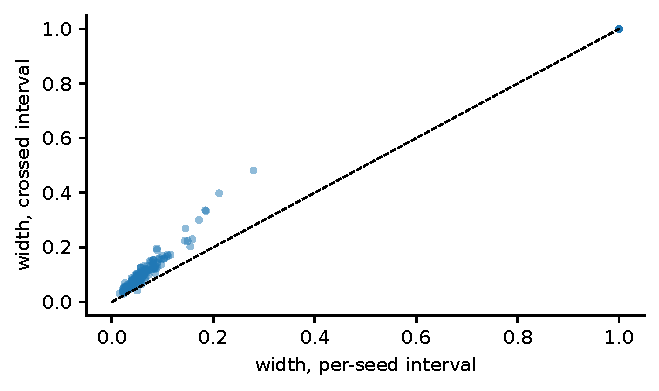
\includegraphics[width=0.55\linewidth]{figures/width_scatter.pdf}
\caption{Width of each corrected interval against the archived one (dashed: equal width).}\label{fig:width}\end{figure}
\begin{table}[H]\centering\scriptsize
\caption{Verdict changes among intervals that concern masking, the primary family, natural test sets, fine-tuning and the transplant. Only the corrected interval is shown; the archived interval is in the comparison file.}\label{tab:corrclaims}
\begin{tabular}{p{4.6cm}p{5.2cm}p{3.4cm}c}\toprule
Result & Row & Corrected estimate [95\% CI] & Significance \\\midrule
PRIMARY\_\allowbreak{}CLAIMS.csv & P2 U-MtE (protected) > mask | Capsule & $-0.006$ [$-0.018, +0.006$] & lost \\
PRIMARY\_\allowbreak{}CLAIMS.csv & P4 U-MtE+balanced > balanced | Ovary & $+0.031$ [$-0.014, +0.077$] & lost \\
adhoc\_\allowbreak{}bootstraps.json & sweep | capsule\_\allowbreak{}dino518 | r=1.0 | umte\_\allowbreak{}balanced-balanced & $+0.057$ [$-0.008, +0.121$] & lost \\
thyroid/\allowbreak{}convnext384\_\allowbreak{}universal & trapA | mask | clean | mask | erm & $+0.021$ [$-0.000, +0.041$] & lost \\
synthetic/\allowbreak{}isic2018/\allowbreak{}dino518\_\allowbreak{}ruler\_\allowbreak{}fixed\_\allowbreak{}corr\_\allowbreak{}main & 0.25 | mask | erm | test\_\allowbreak{}rev & $-0.059$ [$-0.127, +0.008$] & lost \\
synthetic/\allowbreak{}isic2018/\allowbreak{}dino518\_\allowbreak{}ruler\_\allowbreak{}fixed\_\allowbreak{}occlusion\_\allowbreak{}occlusion & 0.0 | mask | erm | test\_\allowbreak{}uncorr & $+0.036$ [$-0.016, +0.086$] & lost \\
synthetic/\allowbreak{}isic2018/\allowbreak{}dino518\_\allowbreak{}ruler\_\allowbreak{}fixed\_\allowbreak{}occlusion\_\allowbreak{}occlusion & 0.5 | mask | erm | test\_\allowbreak{}uncorr & $+0.041$ [$-0.010, +0.090$] & lost \\
synthetic/\allowbreak{}isic2018/\allowbreak{}dino518\_\allowbreak{}ruler\_\allowbreak{}fixed\_\allowbreak{}occlusion\_\allowbreak{}occlusion & 0.75 | mask | erm | test\_\allowbreak{}uncorr & $+0.037$ [$-0.013, +0.086$] & lost \\
synthetic/\allowbreak{}isic2018/\allowbreak{}dino518\_\allowbreak{}ruler\_\allowbreak{}fixed\_\allowbreak{}occlusion\_\allowbreak{}occlusion & 1.0 | mask | erm | test\_\allowbreak{}uncorr & $+0.039$ [$-0.010, +0.091$] & lost \\
synthetic/\allowbreak{}isic2018/\allowbreak{}dino224\_\allowbreak{}ruler\_\allowbreak{}fixed\_\allowbreak{}corr\_\allowbreak{}main & 0.25 | mask | erm | test\_\allowbreak{}rev & $-0.049$ [$-0.117, +0.018$] & lost \\
synthetic/\allowbreak{}thyroid/\allowbreak{}medsiglip448\_\allowbreak{}caliper\_\allowbreak{}corr\_\allowbreak{}main & 1.0 | mask | erm | test\_\allowbreak{}rev & $+0.044$ [$-0.011, +0.104$] & lost \\
synthetic/\allowbreak{}ovary/\allowbreak{}dino518\_\allowbreak{}caliper\_\allowbreak{}corr\_\allowbreak{}main & 0.5 | mask | erm | test\_\allowbreak{}rev & $-0.107$ [$-0.269, +0.054$] & lost \\
capsule/\allowbreak{}dinol518\_\allowbreak{}scale & trapA | mask | clean | mask | erm & $+0.012$ [$-0.006, +0.031$] & lost \\
spec\_\allowbreak{}e13/\allowbreak{}dino518\_\allowbreak{}matched05 & trapA | mask | clean | all | mask | erm & $-0.026$ [$-0.053, +0.000$] & lost \\
spec\_\allowbreak{}e13/\allowbreak{}dinos518\_\allowbreak{}spec\_\allowbreak{}scale & trapB | mask | clean | all | mask | erm & $+0.028$ [$-0.000, +0.055$] & lost \\
spec\_\allowbreak{}e13/\allowbreak{}dinol518\_\allowbreak{}spec\_\allowbreak{}scale & trapA | mask | test\_\allowbreak{}rev | HAM | mask | erm & $-0.044$ [$-0.090, +0.002$] & lost \\
spec\_\allowbreak{}e13/\allowbreak{}dinol518\_\allowbreak{}spec\_\allowbreak{}scale & trapB | mask | clean | all | mask | erm & $-0.025$ [$-0.055, +0.003$] & lost \\
spec\_\allowbreak{}e13/\allowbreak{}dino518\_\allowbreak{}spec\_\allowbreak{}universal & trapA | mask | clean | all | mask | erm & $-0.023$ [$-0.045, -0.001$] & gained \\
spec\_\allowbreak{}e13/\allowbreak{}dino518\_\allowbreak{}spec & trapA | mask | clean | all | mask | erm & $-0.023$ [$-0.045, -0.001$] & gained \\
spec\_\allowbreak{}e13/\allowbreak{}dino518\_\allowbreak{}spec\_\allowbreak{}ablation & trapA | mask | clean | all | mask | erm & $-0.023$ [$-0.045, -0.001$] & gained \\
spec\_\allowbreak{}e13/\allowbreak{}dino518\_\allowbreak{}spec\_\allowbreak{}splice\_\allowbreak{}v2 & trapA | mask | clean | all | mask | erm & $-0.023$ [$-0.045, -0.001$] & gained \\
natural/\allowbreak{}thyroid\_\allowbreak{}dino518\_\allowbreak{}repro/\allowbreak{}natural\_\allowbreak{}boot.json & hard  |  mte-mask & $+0.030$ [$+0.000, +0.061$] & lost \\
natural/\allowbreak{}thyroid\_\allowbreak{}dino518\_\allowbreak{}repro/\allowbreak{}natural\_\allowbreak{}boot.json & easy  |  mask-erm & $+0.042$ [$-0.011, +0.097$] & lost \\
natural/\allowbreak{}isic\_\allowbreak{}MSK\_\allowbreak{}dino518\_\allowbreak{}repro/\allowbreak{}natural\_\allowbreak{}boot.json & all  |  mask-erm & $+0.016$ [$-0.007, +0.038$] & lost \\
natural/\allowbreak{}isic\_\allowbreak{}MSK\_\allowbreak{}dino518\_\allowbreak{}repro/\allowbreak{}natural\_\allowbreak{}boot.json & all  |  balanced-mask & $-0.018$ [$-0.041, +0.005$] & lost \\
finetune/\allowbreak{}thyroid/\allowbreak{}resnet50 & trapA | mte\_\allowbreak{}post | mask\_\allowbreak{}post & $-0.000$ [$-0.001, +0.001$] & lost \\
finetune/\allowbreak{}thyroid/\allowbreak{}resnet50 & trapA | cons\_\allowbreak{}ft | mask & $+0.042$ [$+0.011, +0.074$] & gained \\
finetune/\allowbreak{}thyroid/\allowbreak{}resnet50 & trapB | mte\_\allowbreak{}ft | mask & $-0.042$ [$-0.089, +0.003$] & lost \\
finetune/\allowbreak{}thyroid/\allowbreak{}resnet50 & trapB | mask\_\allowbreak{}balanced | balanced & $+0.069$ [$-0.004, +0.143$] & lost \\
finetune/\allowbreak{}thyroid/\allowbreak{}vit\_\allowbreak{}small\_\allowbreak{}patch16\_\allowbreak{}224.augreg\_\allowbreak{}in21k\_\allowbreak{}ft\_\allowbreak{}in1k & trapA | mask\_\allowbreak{}balanced | balanced & $+0.059$ [$+0.003, +0.122$] & gained \\
finetune/\allowbreak{}thyroid/\allowbreak{}vit\_\allowbreak{}small\_\allowbreak{}patch16\_\allowbreak{}224.augreg\_\allowbreak{}in21k\_\allowbreak{}ft\_\allowbreak{}in1k & trapA | umte\_\allowbreak{}ft | mte\_\allowbreak{}ft & $+0.032$ [$-0.072, +0.125$] & lost \\
finetune/\allowbreak{}capsule/\allowbreak{}resnet50 & trapB | mte\_\allowbreak{}ft | erm & $+0.120$ [$+0.020, +0.217$] & gained \\
review2/\allowbreak{}transplant/\allowbreak{}ovary\_\allowbreak{}dino518 & 0.0 | balanced | erm | test\_\allowbreak{}rev & $+0.019$ [$-0.006, +0.046$] & lost \\
\bottomrule\end{tabular}
\end{table}


\section{What failed or changed}
\begin{itemize}[leftmargin=*]\itemsep1pt
\item \textbf{The transplant ``harm'' is mostly a paste effect.} Earlier drafts quoted the pasted-hair effect as the
harm of masking with in-lesion hair; that attribution is withdrawn. Only N3 is attributed to the artifact, and it is
significant for hair and thyroid only.
\item \textbf{Capsule cannot be matched} under the registered rule; its crossover is descriptive.
\item \textbf{The bootstrap correction} changed \sFourCChanged{} verdicts, and the claims above were rewritten.
\item \textbf{The capsule synthetic cohort did not reproduce its split}; its point estimates moved by up to
\sFourCapMaxDiff, while the location interaction kept its sign and significance.
\end{itemize}

\section{Conclusion}
\textbf{Supported.} The real-artifact crossover is not explained by measured covariates: it survives matching (M1,
3 of 3 feasible cohorts) and doubly robust adjustment (A2, \sFourNATwoOK{} of \sFourNATwo, Holm). Moving the same real
artifact inside the ROI changes what masking does, and for hair and thyroid calipers the artifact's content adds to the
effect of the paste. \textbf{Qualified.} Most of the transplant interaction is produced by the paste itself;
unmeasured confounding of the natural location cannot be excluded. \textbf{Not supported.} A causal harm figure for
the real artifact from the transplant; the capsule matched analysis.

\section{Questions for the supervisor}
\begin{enumerate}\itemsep1pt
\item Is matching plus A2 plus the transplant sufficient causal evidence for a Q1 journal, or should an
instrumental or negative-control analysis be attempted?
\item How should the paper present the paste effect: as a limitation of the transplant, or as a finding in itself
(any label-correlated pattern inside the ROI defeats masking)?
\item Should the full old-versus-new interval table be published as supplementary material?
\end{enumerate}

\section{Next stage}
Stage~5 moves from trap environments to practice: natural test sets without an imposed correlation, clinical
operating points, the thyroid subgroup of 78 patients, the breadth of replication across encoders and fine-tuning,
the DermLIP exception, and a theory judged by its held-out prediction error.

\bibliographystyle{plainnat}
\bibliography{../common/references}
\end{document}
